\documentclass[a4paper, 11pt]{article}           %{{{1
% basic packages                                  {{{2
\usepackage[T1]{fontenc}
\usepackage[scaled=0.975]{helvet}
\usepackage[utf8]{inputenc}
\usepackage{amsmath}
\usepackage{lastpage}
\usepackage{graphicx}
\usepackage{amsfonts}
\usepackage{variations}
\usepackage{pgf,tikz}           % dessin
\usepackage{mathrsfs}
\usetikzlibrary{arrows}
\usepackage{pgfkeys}        % fenetrage des plot TikZ
\usepackage{yhmath}         % arc au dessus des lettres
\usepackage{calc}           % calcul de longueur
\usepackage{variations}     % tableau de variations
\usepackage{multicol}
\usepackage{enumitem}
\usepackage{tcolorbox}                                                          % encadrement texte
% ==== PROGRAMMATION
\usepackage{xcolor}                                                             %
\usepackage{listings}                                                           %
% listings                                        {{{3
\definecolor{mygreen}{rgb}{0,0.6,0}
\definecolor{mygray}{rgb}{0.5,0.5,0.5}
\definecolor{mymauve}{rgb}{0.58,0,0.82}
\definecolor{deepblue}{rgb}{0,0,0.5}
\definecolor{deepred}{rgb}{0.6,0,0}
\definecolor{deepgreen}{rgb}{0,0.5,0}
\lstset{%
% backgroundcolor=\color{white},   % choose the background color; you must add \usepackage{color} or \usepackage{xcolor}; should come as last argument
  basicstyle=\footnotesize,          % the size of the fonts that are used for the code
% breakatwhitespace=false,         % sets if automatic breaks should only happen at whitespace
% breaklines=true,                 % sets automatic line breaking
% captionpos=b,                    % sets the caption-position to bottom
  commentstyle=\color{mygreen},    % comment style
% deletekeywords={type},           % if you want to delete keywords from the given language
% emph={},                         % Custom highlighting
% emphstyle=\ttb\color{deepred}    % Custom highlighting style
% escapeinside={\%*}{*)},          % if you want to add LaTeX within your code
% extendedchars=true,              % lets you use non-ASCII characters; for 8-bits encodings only, does not work with UTF-8
  frame=shadowbox,                 % adds a frame around the code {single, shadowbox}
% keepspaces=true,                 % keeps spaces in text, useful for keeping indentation of code (possibly needs columns=flexible)
  keywordstyle=\color{blue},       % keyword style
  language=C,                      % the language of the code {Python, C}
% morekeywords={*,...},            % if you want to add more keywords to the set
  numbers=left,                    % numbers = (none, left, right)
% numbersep=5pt,                   % how far the line-numbers are from the code
% numberstyle=\tiny\color{mygray}, % the style that is used for the line-numbers
% otherkeywords={self},            % Add keywords here
% rulecolor=\color{black},         % if not set, the frame-color may be changed on line-breaks within not-black text (e.g. comments (green here))
  rulesepcolor=\color{gray}        % shadowbox color
% showspaces=false,                % show spaces everywhere adding particular underscores; it overrides 'showstringspaces'
% showstringspaces=false,          % underline spaces within strings only
% showtabs=false,                  % show tabs within strings adding particular underscores
% stepnumber=1,                    % the step between two line-numbers. If it's 1, each line will be numbered
% stringstyle=\color{mymauve},     % string literal style
% tabsize=4,                       % sets default tabsize to 2 spaces
% title=\lstname                   % show the filename of files included with \lstinputlisting; also try caption instead of title
}
%}}}
%}}}

% mise en page                                    {{{2
\addtolength{\voffset}{-1.8cm}
\addtolength{\textheight}{4cm}
\addtolength{\hoffset}{-2.5cm}
\addtolength{\textwidth}{4cm}
\addtolength{\headsep}{-0.5cm}
\usepackage{fancyhdr}
\setlength{\headheight}{14.00pt}
\pagestyle{fancy} % Numérotation des pages
\renewcommand\headrulewidth{1pt}
\renewcommand\footrulewidth{1pt}
\fancyhead[L]{BP SN}
\fancyhead[C]{arduino}
\fancyhead[R]{détecteur de flamme et buzzer}
\fancyfoot[L]{v 1.6 -- JB}
\fancyfoot[C]{gestion de l'habitat | detection et sécurité incendie}
\fancyfoot[R]{\thepage/\pageref{LastPage}}
%\lhead{3E}%haut de page gauche
%}}}

% Compteurs:                                     {{{2
\addtocounter{page}{0}
\newcounter{Q}
\newcounter{exoNB}
%}}}

% newcommand                                     {{{2
\newcommand{\question}{\stepcounter{Q} $\boxed{\arabic{Q}}$ }
\newcommand{\reponse}{
\par\nobreak
\noindent\rule{0pt}{1.5\baselineskip}% Provides a larger gap between the preceding paragraph and the dots
{\noindent\makebox[\linewidth]{\dotfill}\endgraf}% ... dotted lines ...
% \bigskip% Gap between dots and next paragraph
}

\newcommand{\objectif}[1]{\textsc{\huge \textbf{Objectif :}\\[2mm] #1} }
\newcommand{\partie}[1]{\textsc{\LARGE #1} }

\newcommand{\ligne}{\underline{\hspace{ \textwidth}} }
\newcommand{\exo}[1]{\stepcounter{exoNB}\textsc{\Large Exercice \arabic{exoNB} -- #1} }
\newcommand{\EXO}[2]{\stepcounter{exoNB}\textsc{\Large Exercice \arabic{exoNB} -- #1} \hfill \textbf{#2 points}}
\newcommand{\pb}[1] {\stepcounter{exoNB}\textsc{\Large Problème \arabic{exoNB} -- #1} }
\newcommand{\PB}[2] {\stepcounter{exoNB}\textsc{\Large Problème \arabic{exoNB} -- #1} \hfill \textbf{#2 points}}
%}}}

% Longueur:                                      {{{2
\newlength{\longueurA}
\newlength{\longueurB}
\setlength{\parindent}{0pt}
\setlength{\parskip}{2pt}
\renewcommand{\baselinestretch}{1}
%}}}

% Divers                                          {{{2
% listings                                        {{{3
%\definecolor{mygreen}{rgb}{0,0.6,0}
%\definecolor{mygray}{rgb}{0.5,0.5,0.5}
%\definecolor{mymauve}{rgb}{0.58,0,0.82}
%\definecolor{deepblue}{rgb}{0,0,0.5}
%\definecolor{deepred}{rgb}{0.6,0,0}
%\definecolor{deepgreen}{rgb}{0,0.5,0}
%\lstset{%
%        backgroundcolor=\color{white},   % choose the background color; you must add \usepackage{color} or \usepackage{xcolor}; should come as last argument
%        basicstyle=\footnotesize,        % the size of the fonts that are used for the code
%        breakatwhitespace=false,         % sets if automatic breaks should only happen at whitespace
%        breaklines=true,                 % sets automatic line breaking
%        captionpos=b,                    % sets the caption-position to bottom
%        commentstyle=\color{mygreen},    % comment style
%        deletekeywords={...},            % if you want to delete keywords from the given language
%        escapeinside={\%*}{*)},          % if you want to add LaTeX within your code
%        extendedchars=true,              % lets you use non-ASCII characters; for 8-bits encodings only, does not work with UTF-8
%        frame=single,                    % adds a frame around the code
%        keepspaces=true,                 % keeps spaces in text, useful for keeping indentation of code (possibly needs columns=flexible)
%        keywordstyle=\color{blue},       % keyword style
%        morekeywords={*,...},            % if you want to add more keywords to the set
%        numbers=left,                    % where to put the line-numbers; possible values are (none, left, right)
%        numbersep=5pt,                   % how far the line-numbers are from the code
%        numberstyle=\tiny\color{mygray}, % the style that is used for the line-numbers
%        rulecolor=\color{black},         % if not set, the frame-color may be changed on line-breaks within not-black text (e.g. comments (green here))
%        showspaces=false,                % show spaces everywhere adding particular underscores; it overrides 'showstringspaces'
%        showstringspaces=false,          % underline spaces within strings only
%        showtabs=false,                  % show tabs within strings adding particular underscores
%        stepnumber=2,                    % the step between two line-numbers. If it's 1, each line will be numbered
%        stringstyle=\color{mymauve},     % string literal style
%        tabsize=4,                       % sets default tabsize to 2 spaces
%        title=\lstname                   % show the filename of files included with \lstinputlisting; also try caption instead of title
%}
%\lstset{%
%        language=Python,                 % the language of the code
%        otherkeywords={self},            % Add keywords here
%        deletekeywords={type},           % if you want to delete keywords from the given language
%        emph={},                         % Custom highlighting
%        emphstyle=\ttb\color{deepred}    % Custom highlighting style
%}
%}}}

% PRL style line                                 {{{3
\newlength{\diamondrulelength}
\setlength{\diamondrulelength}{0.6\textwidth}
\newlength{\diamondrulethickness}
\setlength{\diamondrulethickness}{2pt}
\newcommand{\diamondrule}{\begin{center}\tikz{\fill[black] (0.5\diamondrulelength,0) -- (0,0.5\diamondrulethickness) -- (-0.5\diamondrulelength,0) -- (0,-0.5\diamondrulethickness) -- cycle;}\end{center}}
%}}}

% fixed with tabular                             {{{3
\usepackage{array}
\newcolumntype{L}[1]{>{\raggedright\let\newline\\\arraybackslash\hspace{0pt}}m{#1}}
\newcolumntype{C}[1]{>{\centering\let\newline\\\arraybackslash\hspace{0pt}}m{#1}}
\newcolumntype{R}[1]{>{\raggedleft\let\newline\\\arraybackslash\hspace{0pt}}m{#1}}
%}}}

%}}}
%}}}

\begin{document}
\sffamily
\hfill Nom : {\noindent\makebox[5cm]{\dotfill}\endgraf}

\objectif{Détection de flamme et alarme}

Le détecteur de flamme (diode de réception infrarouge) peut être utilisé sur des robots pour trouver la source d'incendie. Ce capteur a une sensibilité élevée à la flamme. Sa photo est dans la figure 1.
\begin{figure}[!h]
\begin{center}
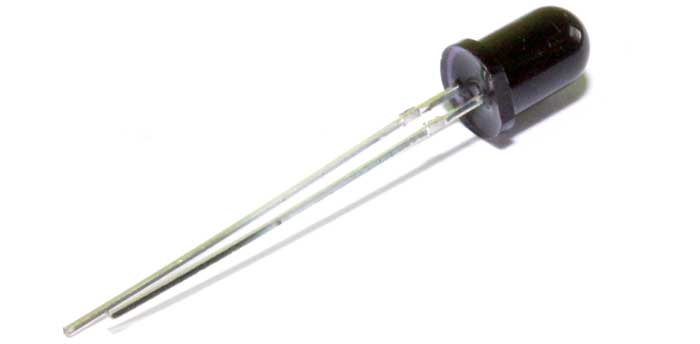
\includegraphics[width=.65\textwidth]{detecteur_flamme}
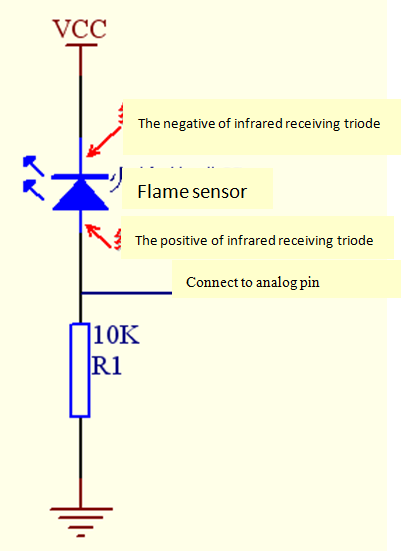
\includegraphics[width=.3\textwidth]{DiodeCircuit}
\label{FigDiodeFlamme}
\caption{Diode infrarouge détectrice de flamme}
\end{center}
\end{figure}


Principe de fonctionnement:\\
Le détecteur de flamme est basé sur le principe selon lequel les rayons infrarouges sont très sensibles aux flammes. Il dispose d'un tube de réception infrarouge spécial conçu pour détecter le feu, puis convertir la luminosité de la flamme en un signal de niveau fluctuant. Les signaux sont ensuite introduits dans le processeur central et traités en conséquence.\\

Connexion du capteur:\\
La broche la plus courte de la diode réceptrice est négative, l'autre positive. Connectez la négative à la broche 5V, positive à la résistance. Connectez l'autre extrémité de la résistance à la masse. Connectez l'extrémité de la diode à la broche analogique A0, comme indiqué sur la figure 1.\\


\partie{Materiel}                         %{{{1
\begin{multicols}{2}
Arduino Board *1\\
USB Cable *1\\
Flame Sensor *1 \\
Active Buzzer*1\\
10K$\Omega$ Resistor*1\\
Breadboard Jumper Wires\\
\end{multicols}

%}}}

\bigskip

\partie{Réalisation} \\                      %{{{1
\begin{figure}[p]
\begin{center}
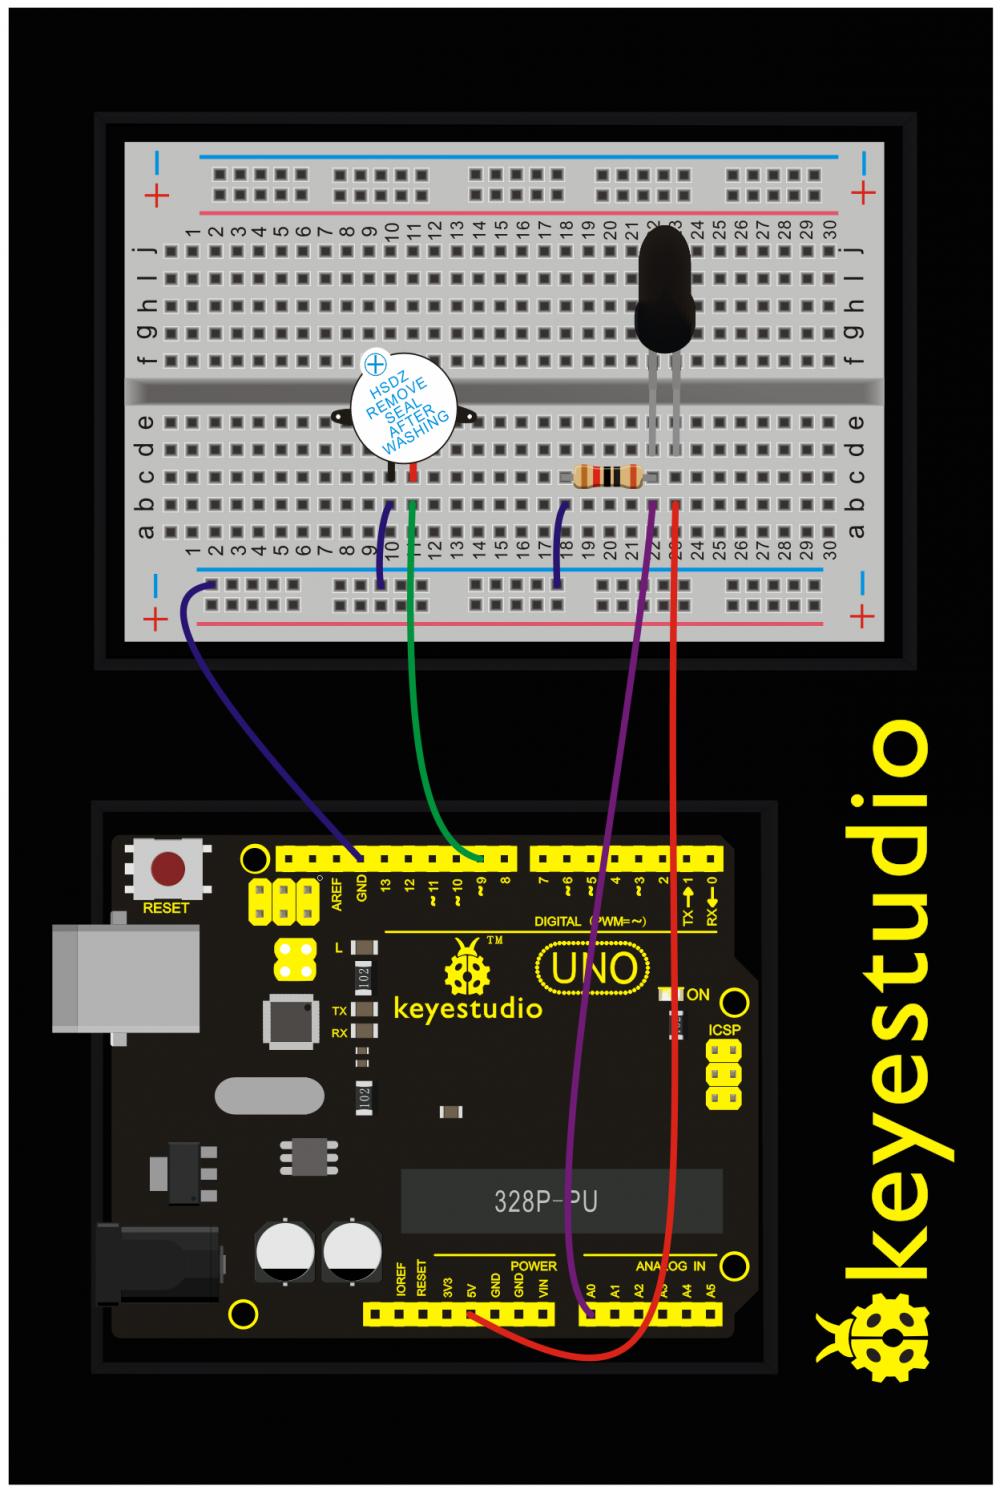
\includegraphics[height=0.9\textheight]{cablage}
\caption{Cablage de la diode détectrice de flamme et du buzzer.}
\label{FigDiodeFlamme}
\end{center}
\end{figure}

Quand la diode s'approche d'un feu, la valeur de tension que lit le port analogique varie. Si vous utilisez un multimètre, la tension qu'il lit est d'environ 0,3V quand il n'y a pas d'incendie. Quand il y a un feu, la tension qu'il lit est de l'ordre de 1.0V. Plus le feu est proche, plus la tension est élevée.
Donc, au début du programme, vous pouvez initialiser la valeur de tension i (pas de feu). Ensuite, vous lisez en continu la valeur de tension analogique j et obtenez la valeur de différence k = j-i. Comparez k avec 0.6V (123 en binaire) pour déterminer si la diode est proche d'un feu ou non. Si oui, le buzzer va sonner.

\question Réalisez le montage.

\question Est-ce que la diode est un composant passif ou actif ?
\reponse

\question Avec un multimètre, mesurez la valeur du potentiel du fil branché à A0 sans flamme ?  \footnote{la masse du multimètre est référencée à celle de la carte arduino}
\reponse

\question Quelle est la valeur de ce potentiel en présence de flamme ?
\reponse

\question Comment est-ce que le microcontrolleur peut il donc détecter la présence de flamme pour faire sonner le buzzer ?
\reponse

\question Quelle est sa valeur lorsque la flamme est très proche (soyons raisonable) ?
\reponse

\question Réprennez les questions 3 et 4 avec une résistance de 5k$\Omega$ et répondezy ci-après. Donnez donc trois valeurs de tension.
\reponse
\reponse
\reponse

\tcbox{\textbf{Constatation professeur :} \hspace{5cm} } % package tcolorbox

\question Expliquez le principe à l'origine de ce changement.
\reponse

\question Trouvez sur internet un produit où cette diode est montée dans une carte d'évaluation, ou breakout board en anglais. Est ce que l'utilisation d'une telle carte nous éviterait de calculer et optimiser le choix de la résistance discutée dans les questions précédentes.
\reponse


\question Quel est la différence entre un buzzer actif et un buzzer passif ?
\reponse

\question Vérifiez le bon fonctionnement du buzzer actif en le polarisant avec 5V.
\tcbox{\textbf{Constatation professeur :} \hspace{5cm} } % package tcolorbox


\question Implémentez le code ci-dessous et le cablage de la figure 1 :

\begin{lstlisting}
int flame=0;// select analog pin 0 for the sensor
int Beep=9;// select digital pin 9 for the buzzer
int val=0;// initialize variable

void setup() {
  pinMode(Beep,OUTPUT); // set LED pin as 'output'
  pinMode(flame,INPUT); // set buzzer pin as 'input'
  Serial.begin(9600);   // set baud rate at '9600'
 }
void loop() {
  val=analogRead(flame);   // read the analog value of the sensor
  Serial.println(val);     // output and display the analog value
  if(val>=600) {           // when the analog value is larger than 600
    digitalWrite(Beep,HIGH); // the buzzer will buzz
  }
  else {
    digitalWrite(Beep,LOW);
  }
  delay(500);
}
\end{lstlisting}

\tcbox{\textbf{Constatation professeur :} \hspace{5cm} } % package tcolorbox

\question Quelle est la valeur binaire de l'entrée analogique A0 quand on lui applique 0V ?
\reponse

\question Quelle est la valeur binaire de l'entrée analogique A0 quand on lui applique 5V ?
\reponse

\question Quelle est la valeur binaire de l'entrée analogique A0 quand on lui applique 0.6V ?
\reponse

\question Convertir ces valeurs en volt et les comparer avec des mesures au multimètre ?
\reponse

\question Choisir deux valeurs de seuil différentes de la variable \texttt{val} pour détecter deux distances de flamme différentes. Préciser ci dessous les deux valeurs de la variable \texttt{val} et les deux distances observées en centimètres.
\reponse
\reponse
%}}}

\bigskip

\partie{Conception \& réalisation avec un buzzer passif} \\                      %{{{1

\question Mettez en oeuvre un buzzer passif avec une mélodie de votre choix.

\tcbox{\textbf{Constatation professeur :} \hspace{5cm} } % package tcolorbox

\question Expliquez son principe de fonctionnement :
\reponse
\reponse
\reponse
\reponse

%}}}

\end{document}
% vim:fdm=marker :fdl=0:wrap


